\documentclass{bioinfo}
\copyrightyear{2005}
\pubyear{2005}

\begin{document}
\firstpage{1}

\title[RVD2]{RVD2: An ultra-sensitive variant detection model for low-depth targeted next-generation sequencing data}
\author[Sample \textit{et~al}]{Corresponding Author\,$^{1,*}$, Co-Author\,$^{2}$ and Co-Author\,$^2$\footnote{to whom correspondence should be addressed}}
\address{$^{1}$Department of XXXXXXX, Address XXXX etc.\\
$^{2}$Department of XXXXXXXX, Address XXXX etc.}

\history{Received on XXXXX; revised on XXXXX; accepted on XXXXX}

\editor{Associate Editor: XXXXXXX}

\maketitle

\begin{abstract}

\section{Motivation:}
Next-generation sequencing technology is increasingly being used for clinical diagnostic tests. Unlike research cell lines, clinical samples are often genomically heterogeneous due to low sample purity or the presence of genetic subpopulations. However, many variant calling algorithms are optimized to call single nucleotide polymorphisms in homogeneous rather than heterogeneous samples.

\section{Results:}
We present a novel variant calling algorithm that uses a hierarchical Bayesian model to estimate allele frequency and call variants in heterogeneous samples. We show that our algorithm improves upon current classifiers and has higher sensitivity and specificity over a wide range of median read depth and minor allele frequency. We identify five mutations in the PAXP1 gene in a matched clinical breast ductal carcinoma tumor sample; two of which are loss-of-heterozygosity events.

%Unmasked positions has median read depth 51 for control sample, and 69 for case sample (from folder '2013-11-22_HCC1187_PAXIP1_genome_Qsd_0_1'; masked positions has median read depth 52 for control sample, and 70 for case sample( from foler '2013-11-22_HCC1187_PAXIP1_hg19masked_Qsd_0_1')
%We use our algorithm to call variants in a pooled sample of 100 patients with multiple sclerosis and identify novel variants in IL7RA and IL2R.
\section{Availability:}
Text  

\section{Contact:} \href{name@bio.com}{name@bio.com}
\end{abstract}

\section{Introduction}

Text Figure~\ref{fig:01} shows that the above method  Text Text Text Text  Text Text Text Text Text Text  Text Text.  \citep{Bag01} wants to know about �� text follows.

\begin{equation}
\sum x+ y =Z\label{eq:01}
\end{equation}

\section{Approach}

Equation~(\ref{eq:01}) Text Text Text Text Text Text  Text Text Text Text Text Text Text Text Text  Text Text Text Text Text Text. Figure \ref{fig:02} shows that the above method  Text Text Text Text  Text Text Text Text Text Text  Text Text.  \citealp{Boffelli03} might want to know about  text text text text ��


\begin{methods}
\section{Methods}

Text 

\end{methods}

\begin{figure}[!tpb]%figure1
%\centerline{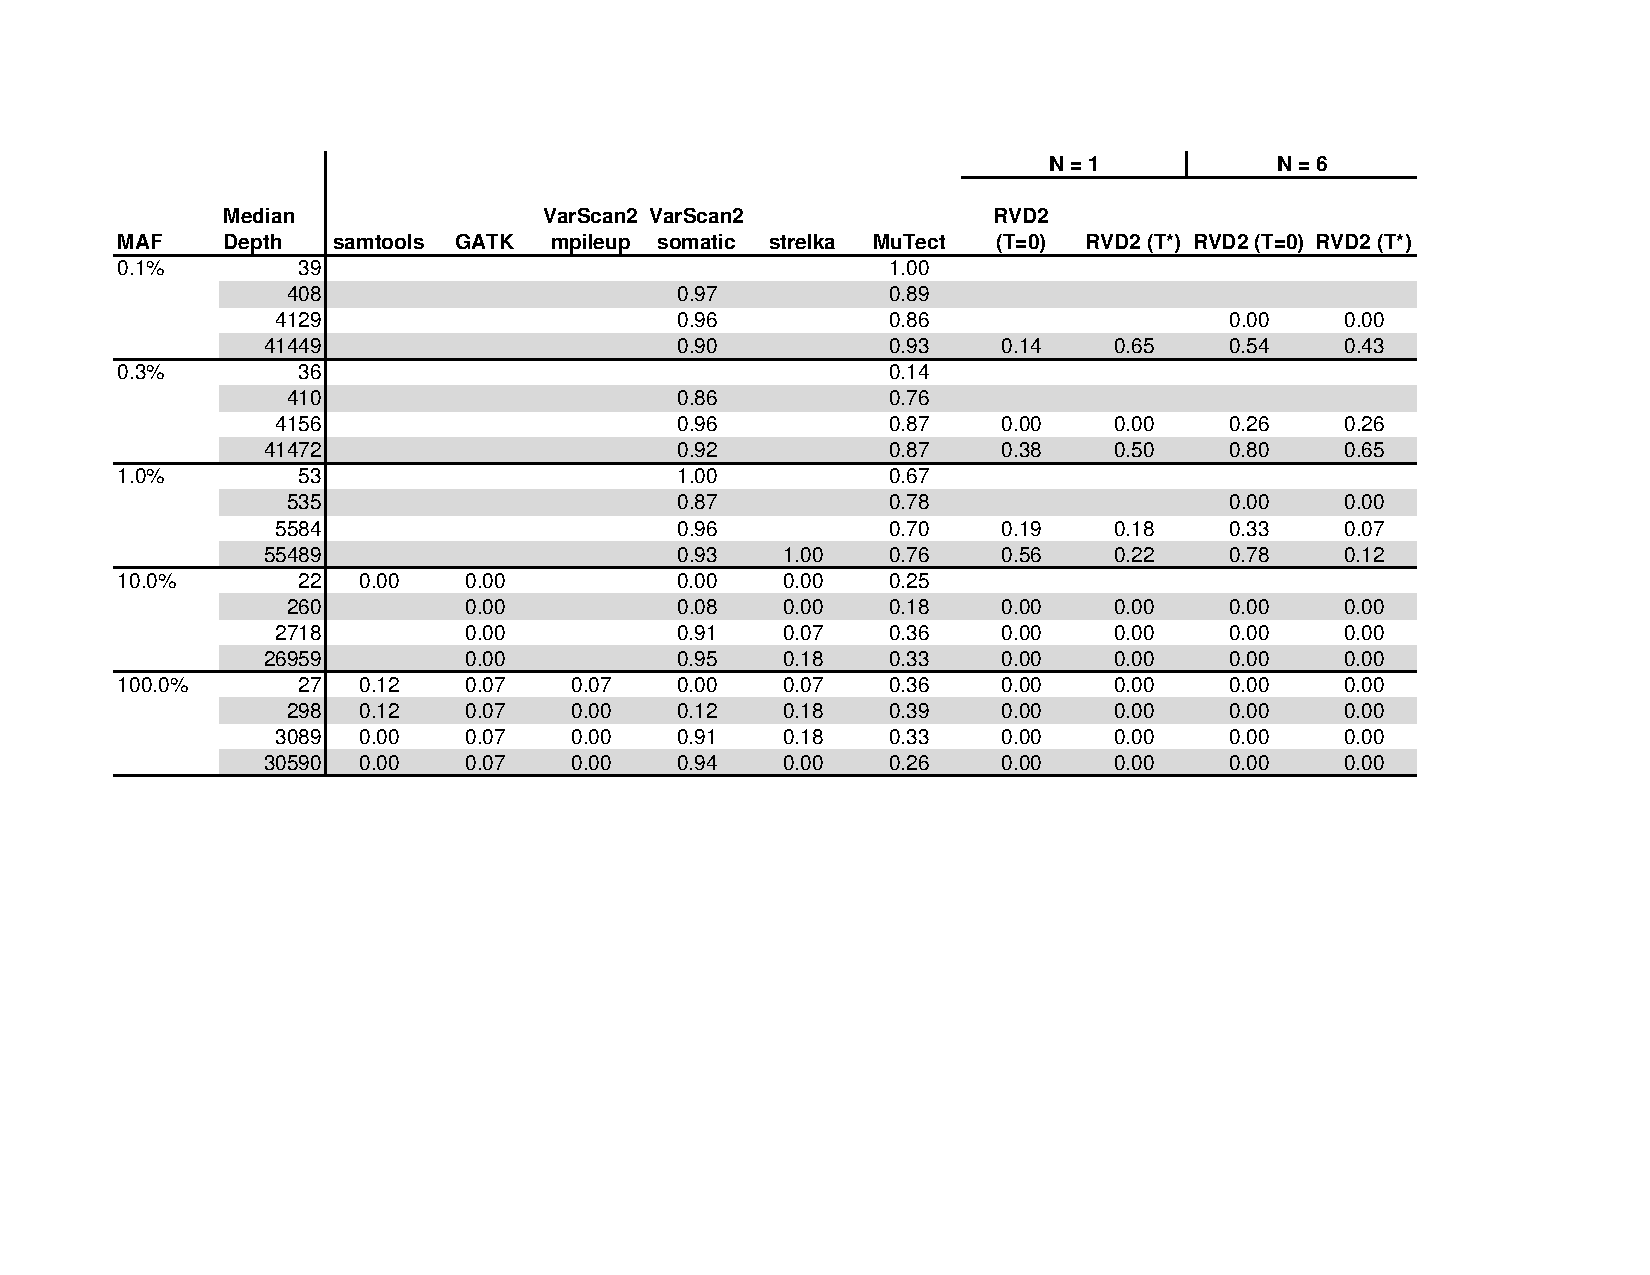
\includegraphics{pdf_figs/comparison_table_fdr.pdf}}
\caption{Caption, caption.}\label{fig:01}
\end{figure}

\begin{figure}[h]
\begin{center}
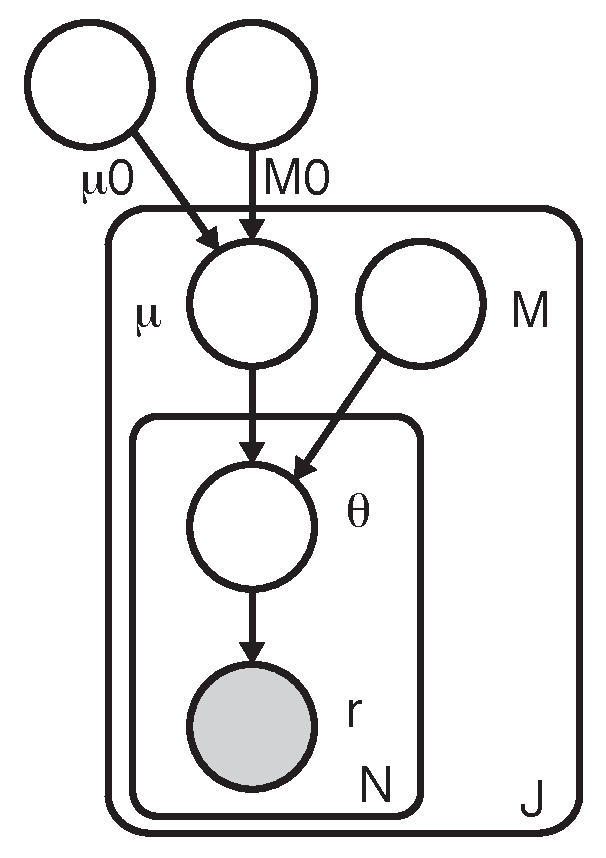
\includegraphics[width=40mm]{pdf_figs/RVD2_model.pdf}
\caption{RVD2 Graphical Model}
\label{fig:graphical_model}
\end{center}
\end{figure}

\section{Discussion}

Text




\section{Conclusion}


\begin{enumerate}
\item this is item, use enumerate
\item this is item, use enumerate
\item this is item, use enumerate
\end{enumerate}


\section*{Acknowledgement}
Text Text Text Text Text Text  Text Text.  \citealp{Boffelli03} might want to know about  text text text text

\paragraph{Funding\textcolon} Text Text Text Text Text Text  Text Text.

%\bibliographystyle{natbib}
%\bibliographystyle{achemnat}
%\bibliographystyle{plainnat}
%\bibliographystyle{abbrv}
%\bibliographystyle{bioinformatics}
%
%\bibliographystyle{plain}
%
%\bibliography{Document}


\begin{thebibliography}{}
\bibitem[Bofelli {\it et~al}., 2000]{Boffelli03} Bofelli,F., Name2, Name3 (2003) Article title, {\it Journal Name}, {\bf 199}, 133-154.

\end{thebibliography}
\end{document}
